\documentclass[svgnames]{article}    

\usepackage{graphicx}                 

% -- math                               
\usepackage{amssymb}
\usepackage{amsmath}
\usepackage{esint}
\usepackage{geometry}

% -- noindent
\setlength\parindent{0pt}

% -- tikz
\usepackage{pgfplots}
\pgfplotsset{compat=1.15}
\usepackage[most]{tcolorbox}

\newtcolorbox{mybox}{
    enhanced,
    boxrule=0pt,frame hidden,
    colback=green!10!white,
    sharp corners
}

% -- figures
\usepackage{float}
\usepackage{caption}
\usepackage{lipsum}
\usepackage{comment}

\usepackage{listings}
\usepackage{xcolor}

\definecolor{codegreen}{rgb}{0,0.6,0}
\definecolor{codegray}{rgb}{0.5,0.5,0.5}
\definecolor{codepurple}{rgb}{0.58,0,0.82}
\definecolor{backcolour}{rgb}{0.95,0.95,0.92}

\lstdefinestyle{mystyle}{
    backgroundcolor=\color{backcolour},   
    commentstyle=\color{codegreen},
    keywordstyle=\color{magenta},
    numberstyle=\tiny\color{codegray},
    stringstyle=\color{codepurple},
    basicstyle=\ttfamily\footnotesize,
    breakatwhitespace=false,         
    breaklines=true,                 
    captionpos=b,                    
    keepspaces=true,                 
    numbers=left,                    
    numbersep=5pt,                  
    showspaces=false,                
    showstringspaces=false,
    showtabs=false,                  
    tabsize=2
}

\lstset{style=mystyle}

% -- start 
\title{Solving the Stochastic Liouville Equation}
\author{Deval Deliwala}
%\date{}                              

\begin{document}
\maketitle
%\tableofcontents    

In our previous notes, we derived the spin Hamiltonian $\mathcal{H}$ for 4H-Silicon
Carbide, which captures the principal spin interactions when 4H-SiC is subjected
to an external magnetic field. We then computed eigenspectra for several model
Hamiltonians, including the complete $16\times16$ representation of
$\mathcal{H}$. \\

Now, our goal is to build a first-principles model of Electrically-Detected Magnetic
Resonance (EDMR) and Near-Zero Field Magnetic Resonance (NZFMR). Specifically,
we want to reproduce the experimental trace shown in Figure \ref{EDMR} using
simulation. 

\begin{figure}[H]
  \centering
    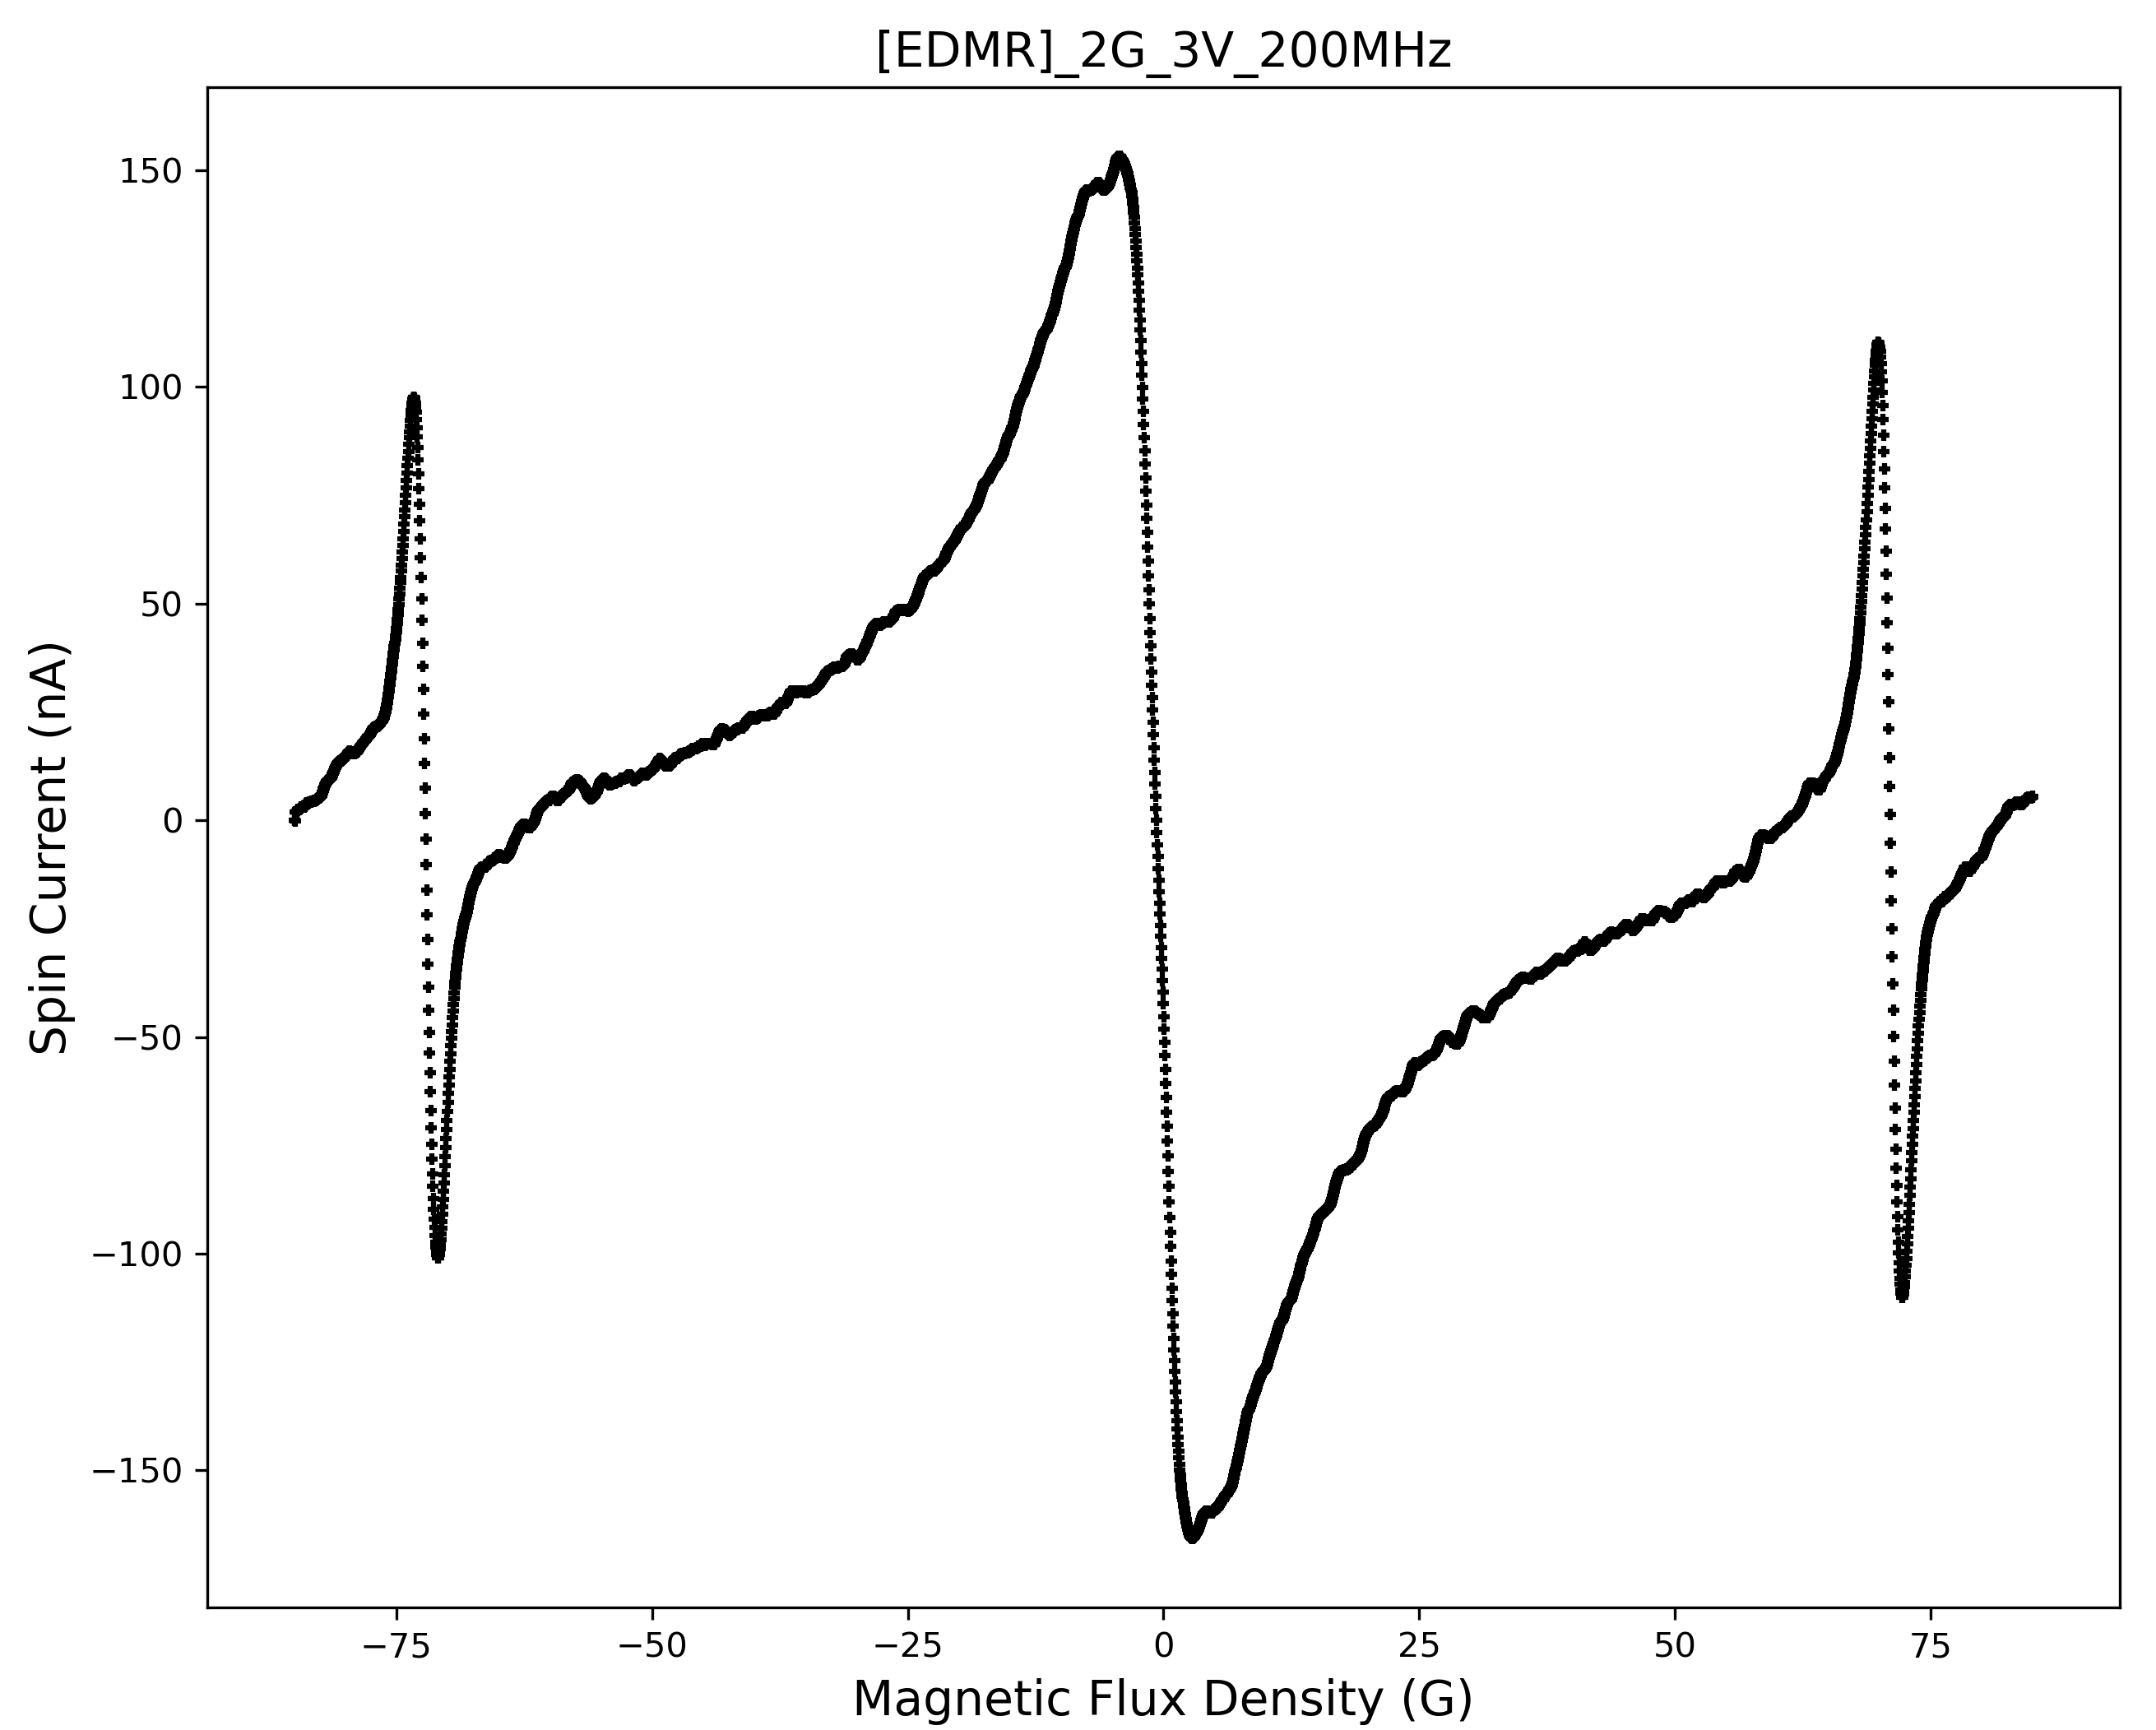
\includegraphics[width=12cm]{EDMR.png}
    \caption{$I$ (nA) vs.\ $B$ (G) EDMR spectra for 4H-SiC at 2~G modulation
    amplitude, 200~MHz, and 3~V bias.}
    \label{EDMR}
\end{figure}

To achieve this, the model must accept both the intrinsic Hamiltonian parameters
(Zeeman, hyperfine, zero‐field splitting, exchange) and the experimental
conditions (bias voltage, modulation amplitude, etc.) as inputs. Next, we specify
the magnetic field range via a tuple $(B_{\mathrm{min}}, B_{\mathrm{max}})$ and
perform the sweep to reproduce the reference spectrum precisely. The framework
should remain flexible, allowing substitution of other experimental
parameters. This will be a long battle, so I will split up this note into
three documents: 

\begin{itemize}
    \item[1.] Solving the Stochastic Liouville Equation (SLE). 
    \item[2.] Building the EDMR model. 
    \item[3.] Least Squares + MCMC fitting the EDMR model. 
\end{itemize}

\tableofcontents 

\newpage
\section{The Stochastic Liouville Equation}

\subsection{Density Matrix Formalism}

The time evolution of a wave function $|\psi\rangle$ is calculated by solving
the time-dependent Schr\"odinger equation: 

\begin{align}\label{schr}
    |\Psi(t)\rangle = e^{\left( -\frac{i}{\hbar}\hat{\mathcal{H}}t\right)}
    |\psi\rangle. 
\end{align}

The \textit{density operator} is defined as 

\begin{align}\label{densop}
\hat{\rho}(t) = \sum_{i}^{} W_i |\Psi_i(t)\rangle \langle \Psi_i(t)|
\end{align} 

where $W_i$ represents the statistical weight of being in the state
$|\Psi_i\rangle$ within the system. In an orthonormal basis $\{\phi_i\}$, the
\textit{density matrix} is given by 

\begin{align}\label{densmat}
    \rho_{i,\,j} = \langle\phi_i | \hat{\rho} | \phi_j\rangle. 
\end{align} 

\subsection{Quantum Liouville Equation}

The \textit{Quantum Liouville Equation} (QLE) is just the Schr\"odinger equation but
in density matrix representation. \\ 

Substituting Equation \ref{schr} into Equation \ref{densop}, we get 

\begin{align} \label{}
    \hat{\rho}(t) &= \sum_{i}^{} W_i e^{\left( -\frac{i}{\hbar}\hat{\mathcal{H}}t
\right)} |\psi_i\rangle \langle \psi_i|
e^{\left(\frac{i}{\hbar}\hat{\mathcal{H}}t\right)}\\
                  &= \sum_{i}^{} W_i \hat{\mathcal{U} }(t) |\psi_i\rangle
                  \langle \psi_i | \hat{\mathcal{U}}^\dagger (t)
\end{align}

Considering an orthonormal basis, we get the time-dependent density matrix from
Equation \ref{densmat}: 

\begin{align}\label{timedens}
    \rho(t) &= \hat{\mathcal{U}}(t) \rho \hat{\mathcal{U}}^\dagger (t) \\
                  &= e^{\left( -\frac{i}{\hbar}\hat{\mathcal{H} }t
                  \right) } \;\rho\; e^{\left(
                      \frac{i}{\hbar}\hat{\mathcal{H} t} \right)  }   
\end{align}

The QLE, describes the time evolution of the density
ensemble can be found by taking the derivative of Equation \ref{timedens} w.r.t
time: 

\begin{align} \label{}
    i\hbar \frac{\partial }{\partial t} \rho(t) 
    &= i\hbar \frac{\partial
    \hat{\mathcal{U} }(t)}{\partial t} \rho \hat{\mathcal{U} }^\dagger(t) + i\hbar
    \hat{\mathcal{U} }(t) \rho \frac{\partial \hat{\mathcal{U} }^\dagger(t)}{\partial t}
    \\
    i\hbar \frac{\partial }{\partial t} \rho(t) &= i\hbar \frac{\partial
    e^{\left( -\frac{i}{\hbar}\hat{\mathcal{H}}t\right)  }}{\partial t} \rho
    \hat{\mathcal{U} }^\dagger (t) + i\hbar \hat{\mathcal{U} }(t) \rho
    \frac{\partial e^{\left( \frac{i}{\hbar}\hat{\mathcal{H} }t \right)
    }}{\partial t}\\ 
    i\hbar \frac{\partial }{\partial t} \rho(t) &= \hat{\mathcal{H} }\left(
    \hat{\mathcal{U} }(t) \rho \hat{\mathcal{U} }^\dagger (t) \right) + \left(
\hat{\mathcal{U} }(t) \rho \hat{\mathcal{U} }^\dagger (t) \right)
\hat{\mathcal{H} } \\  
        i\hbar \frac{\partial }{\partial t} \rho(t) &= \hat{\mathcal{H}
        }(\rho(t)) + (\rho(t)) \hat{\mathcal{H} } \\ 
        i\hbar \frac{\partial }{\partial t} \rho(t) &= \left[ \hat{\mathcal{H} },
        \rho(t) \right].
\end{align}

This equation describes the unitary, non-dissipative evolution of the spin ensemble.
To include environmental interactions, we must generalize to the Stochastic Liouville
Equation (SLE): 

\begin{align} \label{sle}
    \frac{\partial \rho}{\partial t} = -\frac{i}{\hbar}[\mathcal{H}, \,\rho] -
    \frac{k}{2}\{ \Lambda, \,\rho \} + p\Gamma. 
\end{align}

The first term on the right-hand side reproduces the unitary QLE.  
The second term introduces dissipation: at rate $k$, the projection operator
$\Lambda$ removes spin pairs from the corresponding subspace.  
The third term acts as a source, injecting spin pairs with random orientations
at rate $p$.  Here, $\Gamma$ denotes the $16\times16$ identity matrix.  This
formulation provides the basis for computing the various spin–spin reactions
that give rise to the observed EDMR and NZFMR spectra. \\

By substituting our full spin Hamiltonian into Equation \ref{sle} and applying
a small modification, we capture spin-dependent recombination (SDR) and thus
derive a model for EDMR and NZFMR simulations. \\

We adopt the modified SLE of Hansen and Pedersen\footnote{%
  https://www.sciencedirect.com/science/article/abs/pii/S0009261402007248?via\%3Dihub%
}:
\begin{align} \label{}
    \frac{\partial \rho}{\partial t}
    = -\frac{i}{\hbar}[\mathcal{H}, \rho]
    - \tfrac{1}{2}(k_S + k_D)\{\Lambda_S, \rho\}
    - \tfrac{1}{2}\,k_D\,\{\Lambda_T, \rho\}
    + \tfrac{1}{16}\,p\,\Gamma.
\end{align}

Again, the first term is the unitary evolution.  
The second term, via $\Lambda_S$, removes singlet states at the effective rate
$(k_S + k_D)$.  
The third term, via $\Lambda_T$, accounts for triplet dissociation into the
conduction band at rate $k_D$.  
The final term injects carriers at rate $p$, with $\Gamma$ the identity; the
factor $1/16$ normalizes this over the 16-dimensional space. \\

Since carrier generation and annihilation proceed at constant rates, we
focus on the steady-state SLE ($\partial\rho/\partial t = 0$). Hence, we solve
\begin{align} \label{}
    0
    &= -\frac{i}{\hbar}[\mathcal{H}, \rho]
       - \tfrac{1}{2}(k_S + k_D)\{\Lambda_S, \rho\}
       - \tfrac{1}{2}\,k_D\,\{\Lambda_T, \rho\}
       + \tfrac{1}{16}\,p\,\Gamma.
\end{align}

\newpage
\section{Solving the Stochastic Liouville Equation}

\subsection{Sylvester Form}

We consider a pair of electrons (spin-$\frac{1}{2}$) coupled to two
spin-$\frac{1}{2}$ nuclei ($^{29}$Si + $^{13}$C). The composite Hilbert space is 

\[
    \mathcal{H} = \left(\frac{1}{2}\text{-electron}\right)^{\otimes 2} \otimes
\left(\frac{1}{2}\text{-nucleus} \right)^{\otimes 2}, \qquad
\text{dim}\mathcal{H} = 2^4 = 16. 
\] \vspace{3px}

We have a symbolically parameterized Spin Hamiltonian (from the previous notes): 

\[
\hat{\mathcal{H}}_\text{sym} \in \mathbb{C}^{16\times 16} 
\] \vspace{3px}

that contains Zeeman, Hyperfine, Zero-field Splitting, and Exchange terms. \\ 

The SDR model augments the unitary QLE-von Neumann equation with three
dissipative channels 

\begin{align} \label{hansped}
    0 = -\frac{i}{\hbar}[\mathcal{H} , \rho] - \frac{1}{2}(k_S + k_D)
    \{\Lambda_S, \rho\} - \frac{1}{2}k_D \{\Lambda_T, \rho\} +
    \frac{1}{16}p\Gamma, 
\end{align} 
where 
\begin{itemize}
    \item[.] $[\mathcal{H} , \rho]$ - coherent precession. 
    \item[.] $\{\Lambda_S, \rho\}$ - recombination of  \textit{singlet} electron
        pairs into the valence band. 
    \item[.] $\{\Lambda_T, \rho\}$ - dissociation of  \textit{triplet} electron
        pairs into the conduction band. 
    \item[.] $\frac{1}{16}p\Gamma$ - spin-pair generation at rate $p$ 
        uniformly over the 16-dimensional space. 
\end{itemize}

Equation \ref{hansped} is a \textit{linear, time-homogeneous, trace
non-conserving} master equation that can be rearranged into a \textbf{Sylvester
Equation.}\\ 

We rewrite Equation \ref{hansped} into Sylvester form (more specifically, a
continuous Lyapunov) via 

\begin{align}\label{sylvfull}
A\rho + \rho A^\dagger + g = 0 
\end{align}

where 

\begin{align} \label{sylv}
    A = -\frac{i}{\hbar}\mathcal{H} - \frac{1}{2}(k_S + k_D) \Lambda_S -
    \frac{1}{2}k_D\Lambda_T, \qquad g = -\frac{1}{16}p\Gamma.
\end{align}

The steady state is a unique solution \textbf{if and only if} $A$ has no purely
imaginary eigenvalues. 

\section{Modeling Sylvester}

The solution of Equation \ref{sylvfull} is given by
\[
    \rho = \int_0^\infty e^{-iA t}\,g\,e^{iA^\dagger t}\,\mathrm{d}t.
\]

Although this integral form is formally exact, numerical implementations
rely on matrix operations.  We therefore vectorize
Equation \ref{sylvfull} into a linear system.\\

We begin by defining a solver class for the steady-state SLE.  The class
accepts the symbolic spin Hamiltonian, the singlet/triplet projectors, and
the $16\times16$ identity matrix $\Gamma$.

\begin{lstlisting}[language=Python]
@dataclass
class SteadyStateSLESolver:
    """
    Build the singlet-triplet Liouvillian for a 2-electron + 2-nucleus (I=1/2)
    spin system numerically. Returns a callable

        rho_numeric(**params) -> 16x16 numpy array (trace=1)

    We use a modified spin-dependent recombination (SDR) model from Hansen
    and Pedersen. The steady-state equation is

        0 = -(i/$\hbar$)[H,$\rho$]
            - 1/2($k_S + k_D$){$\Lambda_S,\rho$}
            - 1/2$k_D${$\Lambda_T,\rho$}
            + (p/16)$\Gamma$.

    Here, $\Lambda_S$ and $\Lambda_T$ project onto the electronic singlet
    and triplet subspaces (with identity on the nuclear sector).  $\Gamma$
    is the 16x16 identity.
    """
    
    H_sym:      sp.Matrix
    Lambda_S:   sp.Matrix | ndarray
    Lambda_T:   sp.Matrix | ndarray
    Gamma:      sp.Matrix | ndarray
    ...
\end{lstlisting}
\vspace{5px}

To convert symbolic \verb|sp.Matrix| objects into numerical
\verb|np.ndarray| matrices, we define a helper that applies a substitution
map \verb|subs| from symbols to float values.

\begin{lstlisting}[language=Python]
def _to_numeric(M: sp.Matrix | ndarray, subs: Mapping[sp.Symbol, float]) -> ndarray:
    """
    Convert a sympy.Matrix into a numpy.ndarray by substituting parameters
    and evaluating numerically.
    """
    if isinstance(M, sp.Matrix):
        return np.array(M.subs(subs).evalf(), dtype=complex)
    return np.array(M, dtype=complex)
\end{lstlisting}
\vspace{5px} 

With this in place, we assemble the Sylvester operator \(A\) and the
generation term \(g\).
\begin{lstlisting}[language=Python]
    # build numerical A operator in Sylvester eq.
    def _build_A(self, *, k_s: float, k_d: float, subs: Mapping[sp.Symbol, float]) -> ndarray:
        H = np.array(self.H_sym.subs(subs).evalf(), dtype=complex)
        LS = np.array(_to_numeric(self.Lambda_S, subs), dtype=complex)
        LT = np.array(_to_numeric(self.Lambda_T, subs), dtype=complex)
        return (
            -(1j / self.hbar) * H
            - 0.5 * (k_s + k_d) * LS
            - 0.5 * k_d * LT
        )
\end{lstlisting}

\begin{lstlisting}[language=Python]
    # generation term
    def _build_g(self, *, p: float, subs: Mapping[sp.Symbol, float]) -> ndarray:
        Gamma = np.array(_to_numeric(self.Gamma, subs), dtype=complex)
        return (p / 16.0) * Gamma
\end{lstlisting}

\subsection{Vectorization}

To turn Equation \ref{sylvfull} into a \emph{linear} problem we
vectorize the density matrix.  Let $\text{vec}(\rho)$ be the
256-component column vector obtained by stacking the
\emph{columns} of~$\rho$.  Using the identity
\[
    \text{vec}(X\rho Y)=\bigl(Y^{T}\otimes X\bigr)\,
    \text{vec}(\rho),
\]%
Equation \ref{sylvfull} becomes
\begin{align}\label{linear}
    \underbrace{\bigl(I\otimes A+A^\dagger\otimes I\bigr)}_{%
    M\in\mathbb{C}^{256\times256}}\,
    \text{vec}(\rho) = -\,\text{vec}(g).
\end{align}
Equation \ref{linear} is a standard linear system that can be solved
with any dense solver. I use \verb|np.linalg.solve| with fortran column
ordering. 

\begin{lstlisting}[language=Python]
    def rho(
        self, *,
        k_s: float,
        k_d: float,
        p: float,
        params: Mapping[str, float] | None = None,
    ) -> ndarray:
        """
        Return the steady-state density matrix (16x16, complex Hermitian).

          * Hamiltonian parameters are supplied through `params`.
          * Kinetic parameters are `k_s`, `k_d`, and `p`.

        Args
        ----
        k_s, k_d : float
            Singlet recombination and triplet dissociation rates (s^-1).
        p : float
            Spin-pair generation rate (s^-1).
        params : dict[str, float], optional
            Numeric values for every free symbol in `H_sym`
            (B0, g_e, mu_B, ...).
        """
        if params is None:
            params = {}
        subs = {sp.Symbol(k): v for k, v in params.items()}
        self._check_param_completeness(subs)

        A = self._build_A(k_s=k_s, k_d=k_d, subs=subs)   # (16, 16)
        self._spectral_check(A)

        B = A.conj().T                                   # (16, 16)

        g = self._build_g(p=p, subs=subs)                # (16, 16)
        I = np.eye(self.N, dtype=complex)                # (16, 16)
        M = kron(I, A) + kron(B.T, I)                    # (256, 256)
        self._structure_checks(M, A, B)

        # solve for vec(rho)
        vec_rho = np.linalg.solve(M, -g.reshape(-1, 1, order="F"))

        # reshape 256x1 ->  16x16 
        rho = vec_rho.reshape(self.N, self.N, order="F")
        rho = self._postprocess(rho)
        return rho
\end{lstlisting}

For any combination of Hamiltonian and experimental parameters
(including a specific magnetic-field value~$B$), calling
\verb|SteadyStateSLESolver.rho(...)| returns the steady-state density
matrix of the full spin ensemble.  To guarantee numerical correctness
the solver performs several checks.

\subsubsection{Checks}

\paragraph{1.~Dimension check.}
Ensure every operator supplied to the solver has the correct
$16\times16$ shape:
\begin{lstlisting}[language=Python]
    def _check_dimensions(self):
        for name, M in (
            ("H", self.H_sym),
            ("Lambda_S", self.Lambda_S),
            ("Lambda_T", self.Lambda_T),
            ("Gamma", self.Gamma),
        ):
            if M.shape != (self.N, self.N):
                raise ValueError(f"{name} must be {self.N}x{self.N}; got {M.shape}.")
\end{lstlisting}

\paragraph{2.~Parameter completeness.}
Confirm the substitution dictionary covers every free symbol:
\begin{lstlisting}[language=Python]
    def _check_param_completeness(self, subs: Mapping[sp.Symbol, float]):
        missing = set(self._free_params) - set(subs)
        if missing:
            raise ValueError(
                "numeric values missing for: " + ", ".join(s.name for s in missing)
            )
\end{lstlisting}

\paragraph{3.~Spectral check.}
The Sylvester equation is solvable only if
$A$ has no eigenvalues with real part~$0$.  A numerical margin of
$10^{-10}$ is enforced:
\begin{lstlisting}[language=Python]
    def _spectral_check(self, A: ndarray):
        lam = eigvals(A)
        if np.any(np.abs(np.real(lam)) < 1e-10):
            raise ValueError(
                "steady state solution must be unique; some eigenvalues are near 0."
            )
        return lam
\end{lstlisting}

\paragraph{4.~Structure check.}
After vectorization we verify the Kronecker-sum matrix,
its rank, and the relation $B=A^\dagger$:
\begin{lstlisting}[language=Python]
    def _structure_checks(self, M: ndarray, A: ndarray, B: ndarray):
        N2 = self.N * self.N  # 256
        if M.shape != (N2, N2):
            raise RuntimeError("Kronecker sum matrix M has wrong dimensions.")
        if np.linalg.matrix_rank(M) < N2:
            raise RuntimeError("M is singular; steady state not unique or absent.")
        if not np.allclose(B, A.conj().T):
            raise RuntimeError("B != A^dagger")
\end{lstlisting}

\paragraph{5.~Post-processing.}
After reshaping the solution back to $16\times16$ we enforce Hermiticity,
normalise the trace, and check positivity:
\begin{lstlisting}[language=Python]
    def _postprocess(self, rho: ndarray) -> ndarray:
        # enforce Hermiticity
        rho = 0.5 * (rho + rho.conj().T)

        # trace normalisation
        tr = np.trace(rho)
        if not np.isclose(tr, 1.0, atol=1e-8):
            rho /= tr

        # positivity (tiny negatives tolerated)
        evals = eigvalsh(rho)
        if np.any(evals < -1e-8):
            raise RuntimeError("rho not positive semi-definite (min eigenvalue < 0).")

        return rho
\end{lstlisting}

The first line explicitly projects out any
anti-Hermitian numerical noise so that $\rho$ is
\emph{exactly} Hermitian before further tests. \\

The resulting $\rho(B)$ is the steady-state solution of
Equation~\ref{sle}.  Sweeping $B$ from $(B_{\text{min}},B_{\text{max}})$
yields the full density matrix—and therefore a complete description of
the spin ensemble—at each field point.

\section{Connecting back to EDMR/NZFMR}

The measured EDMR/NZFMR signal is proportional to the singlet
population in the sample, since only singlets ($S=0$) can recombine by
spin-selection rules (spin angular momentum conservation). Hence, we compute

\[
    P_S(B)=\mathrm{Tr}\bigl(\Lambda_S\,\rho(B)\bigr),
\] \vspace{5px}

where $\Lambda_S$ is the singlet projector on the 16 $\times$ 16 Hilbert space. 
Finally the EDMR and NZFMR spin current can be modeled via

\[
    I(B)\propto P_S(B)
    \quad\Longrightarrow\quad
    I(B)=A\,\mathrm{Tr}\bigl(\Lambda_S\rho(B)\bigr)+I_0,
\] \vspace{5px}

where $A$ is a scaling constant and $I_0$ a small offset.  Determining
$A$ and $I_0$ by fitting will be the subject of a future note.

\end{document}

